\RequirePackage[2020-02-02]{latexrelease}


% Template for seminar reports
% Computer Vision Group, Visual Computing Institute, RWTH Aachen University
\documentclass[twoside,a4paper,article]{combine}
\usepackage[utf8]{inputenc}
\usepackage{a4}
\usepackage{fancyhdr}   
%\usepackage{german}    % Uncomment this iff you're writing the report in German
\usepackage{makeidx}
\usepackage{color}
\usepackage{t1enc}		% German letters in the "\hyphenation" - command
\usepackage{latexsym}	% math symbols
\usepackage{amssymb}    % AMS symbol fonts for LaTeX.
\usepackage{graphicx}
\usepackage{pslatex}
\usepackage{ifthen}
\usepackage{booktabs}
\usepackage[T1]{fontenc}
\usepackage{pslatex}
\usepackage{psfrag}
\usepackage{subfigure}
\usepackage{url}
\usepackage{datetime}
\usepackage{xspace}
\usepackage{newtxmath}

\usepackage{float} %figure inside minipage

\newdateformat{monthyeardate}{\monthname[\THEMONTH] \THEYEAR}

% Do not change these sizes and do not add superfluous 
% pagebreaks to increase the page count.
\setlength{\oddsidemargin}{3.6pt}
\setlength{\evensidemargin}{22.6pt}
\setlength{\textwidth}{426.8pt}
\setlength{\textheight}{654.4pt}
\setlength{\headsep}{18pt}
\setlength{\headheight}{15pt}
\setlength{\topmargin}{-41.7pt}
\setlength{\topskip}{10pt}
\setlength{\footskip}{42pt}
\setlength{\parindent}{0pt}

\makeatletter
\DeclareRobustCommand\onedot{\futurelet\@let@token\@onedot}
\def\@onedot{\ifx\@let@token.\else.\null\fi\xspace}
\def\eg{\emph{e.g}\onedot} \def\Eg{\emph{E.g}\onedot}
\def\ie{\emph{i.e}\onedot} \def\Ie{\emph{I.e}\onedot}
\def\cf{\emph{c.f}\onedot} \def\Cf{\emph{C.f}\onedot}
\def\etc{\emph{etc}\onedot} \def\vs{\emph{vs}\onedot}
\def\wrt{w.r.t\onedot} \def\dof{d.o.f\onedot}
\def\etal{\emph{et al}\onedot}
\makeatother

% =========================================================================
\graphicspath{{pictures/}}
\setcounter{secnumdepth}{3}
\setcounter{tocdepth}{3}

% =========================================================================
\begin{document}
% Template for seminar reports
% Seminar Current Topics in Computer Vision and Machine Learning


\begin{titlepage}
    \begin{center}
    \ 
    \vspace{3.5cm}
    
    \textsf{
    RWTH Aachen University \\
    Faculty of Mathematics, Computer Science and Natural Sciences\\
    Chair of Computer Science 13 (Computer Vision) \\
    Prof. Dr. Bastian Leibe
    }
    
    \rule{\linewidth}{1pt}
    
    \vspace{1.75cm}
    \LARGE
    \textbf{Seminar Report}
    
    \vspace{1.7cm}
    \huge
    Linear and Nonlinear Filters
    
    \vspace{3.0cm}
    \Large
    Alexander Skretting\\
    \large
    Matriculation Number: 445457

    \vspace{1.0cm}
    \Large
    Jose Rigel Soeryo Soebandoro\\
    \large
    Matriculation Number: 444345
    
    \vspace{0.5cm}
    \monthyeardate\today
    
    \vspace{1.05cm}
    \rule{\linewidth}{1pt}
    
    \vspace{0.5cm}
    \textsf{\textbf{
    \normalsize
    \begin{tabular}{ll}
    Advisor:  & George Lydakis\\
    \end{tabular}
    }}
    \end{center}
\end{titlepage}



\begin{abstract}
% +++++++++++++++++++++++++
% Insert your Abstract here (one paragraph summary)
% +++++++++++++++++++++++++
\end{abstract}

\tableofcontents
\newpage
% =========================================================================

\section{Introduction}
\section{Linear Filters}
As its name suggests, the function which is used to pass the image through
must be linear and shift invariant.

A common formula for linear filtering is the \emph{Correlation Filtering}.
\[
    g(i,j) = \sum_{l \in \mathscr{M}}\sum_{k \in \mathscr{N}}{f(i+k, j+l) \cdot h(k, l)}
\]
or commonly notated as $g = f \otimes h$.\hfill\\

The desired output pixel $g(i, j)$, where $i$ and $j$ specify the
coordinates of it, is based on a $M \times N$ sized neighborhood, 
meaning not only does one pixel define an output pixel, but also a specified number
of its neighbors. The influence of each pixel in the neighborhood is defined by the filter coefficient $h(k, l)$,
also called its \emph{kernel} or \emph{mask}.\\

$$
\underbrace{
    \begin{bmatrix}
        128 & 34 & 123\\
        68 & 54 & 73 \\
        100 & 95 & 17
    \end{bmatrix}}_{\text{input neighborhood}}
\otimes
\underbrace{
    \begin{bmatrix}
        0.1 & 0.1 & 0.1\\
        0.1 & 0.2 & 0.1\\
        0.1 & 0.1 & 0.1
    \end{bmatrix}}_{\text{kernel}}
= 75
$$

As the above example with a $3 \times 3$ kernel, a total of 9 pixels is needed to calculate a single output pixel.\\

Another common variant on the formula is having the signs of the offsets reversed. 
\[
    g = f \ast h
\]
\[
    g(i,j) = \sum_{l \in \mathscr{M}}\sum_{k \in \mathscr{N}}{f(i-k, j-l) \cdot h(k, l)}
\]
With this formula, $\ast$ is called the \emph{convolutional} operator, and the kernel $h$ is called the \emph{impulse response function}. An interesting note is that, 
when the kernel $h$ is convolved with an impulse signal $\delta$ (an image with 0 everywhere except the origin),
it reproduces the kernel itself $h \ast \delta = h$, whereas with correlational filtering, it produces the reflected signal (inverted signal in both dimensions).\\

An apparent problem from neighborhood filtering is that on the edges, the neighbors simply does not exist in one or two directions (e.g. a $1000\times1000$ image passed
through a $3\times3$ kernel would produce a $998\times998$ image). There are a couple method to alleviate the calculation of the nonexistent neighbors.

\begin{minipage}{\textwidth}\begin{figure}[H]
    \centering
    \subfigure[zero]{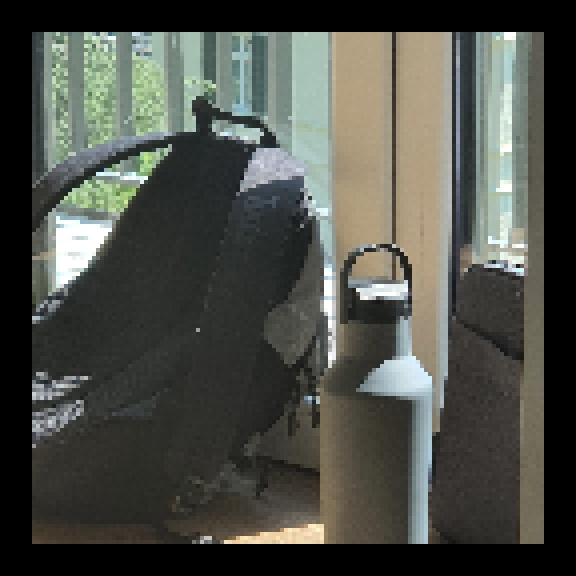
\includegraphics[width=0.24\textwidth]{img/border_constant}}
    \subfigure[wrap]{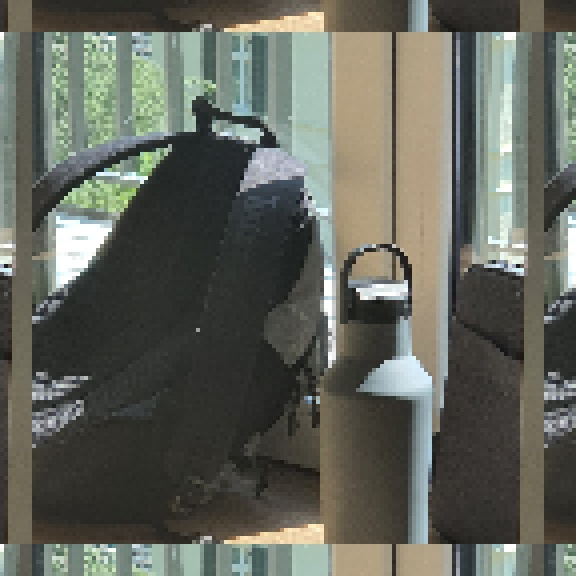
\includegraphics[width=0.24\textwidth]{img/border_wrap}}
    \subfigure[clamp]{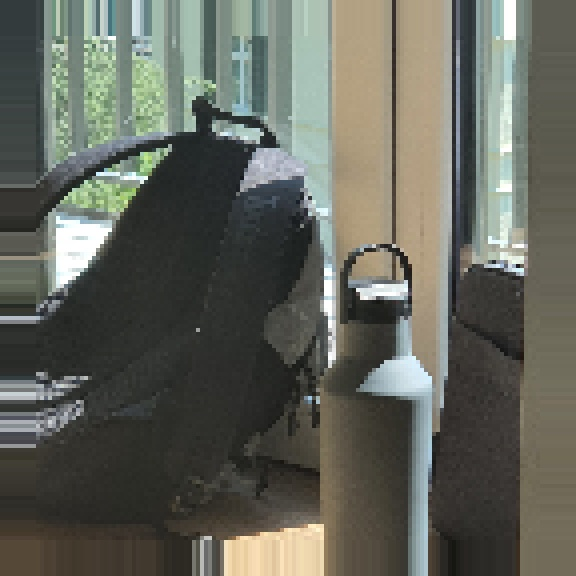
\includegraphics[width=0.24\textwidth]{img/border_clamp}}
    \subfigure[mirror]{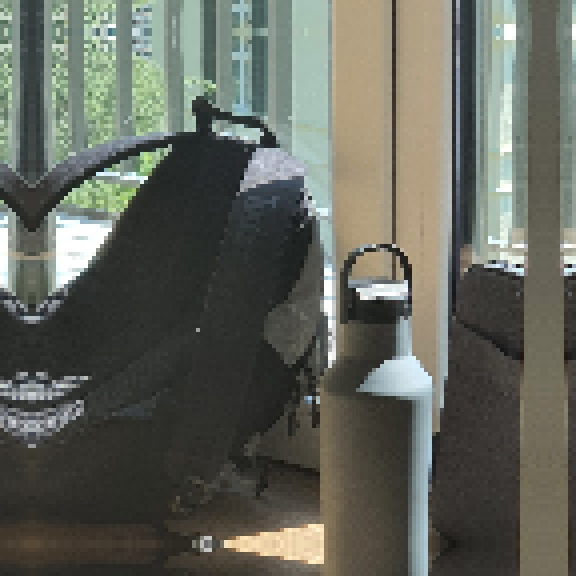
\includegraphics[width=0.24\textwidth]{img/border_reflect}}
    
\end{figure}\end{minipage}


% TEMPLATE EXAMPLES BELOW===========================================
\newpage
\section{example page from template}
Please specify your name, matriculation number, the name of your advisor and the title of your report in 
\verb+titlepage.tex+.

Using BibTeX, you can cite papers in an organized way.
Just enter the information about a paper or an article you want to cite in the \texttt{seminar\_report.bib} file and use \verb+\cite+ to cite them. For example \verb+\cite{Deng09CVPR}+ produces \cite{Deng09CVPR} or \verb+\cite{Kingma14Arxiv}+ for \cite{Kingma14Arxiv}. You can combine multiple citations in one as \verb+\cite{Deng09CVPR,Kingma14Arxiv}+, producing \cite{Deng09CVPR,Kingma14Arxiv}.
Don't forget to compile the bib file and LaTeX will add all the cited references at the end. You can use the provided Makefile for this, or configure your LaTeX editor of choice to do it for you (\eg, TexStudio).
Cite all the literature you use and state where the figures are from! You can use conference and journal name abbreviations in the .bib file, such as CVPR or NeurIPS (see the full list in the \texttt{abbrev.bib} file) or write the full name of the journal or conference.

When a paper has both a published (peer-reviewed) journal/conference version and an ArXiv version, prefer citing the published paper instead of the ArXiv one.

\section{Section Title}
\label{sec:firstsection}
I am a section. LaTeX will give me a number \emph{automatically} and put me into the table of contents.
Using \verb+\label+ and \verb+\ref+ you can write that this is Section \ref{sec:firstsection}. Another section is Section \ref{sec:another}.

You can use the commands \verb+\eg+,  \verb+\ie+,  \verb+\etal+ to get \eg, \ie, \etal. And ``this is a quote.''

\subsection{Subsection Title With Capitalized Words}
We can make bulleted lists as follows.

\begin{itemize}
\item I am an item,
\item I am another item.
\end{itemize}

\subsubsection{Subsubsection with only the first word capitalized}
I am a subsubsection, an even smaller subsection. Let's see a table.

\begin{table}[h]
\centering
\begin{tabular}{lc}
\toprule
Method & Accuracy (\%) \\
\midrule
Boring old method & 86.6 \\
Shiny new method & 86.7 \\
\bottomrule
\end{tabular}
\caption{This is the caption for the table.}
\label{tab:mytable}
\end{table}

Tab.~\ref{tab:mytable} is an example table. The table also got a number automatically and will be placed where LaTeX thinks it looks good. You can specify a preference with h(ere), t(op), b(ottom), p(age).

\section{Another Section}
\label{sec:another}

\begin{figure}[h]
\centering
\caption{Insert caption here. Image from~\cite{Deng09CVPR}.}
\label{fig:example_figure}
\end{figure}

% Similarly to tables, we can also create figures. Fig.~\ref{fig:example_figure} also got a number.

\section{Equations}
LaTeX is also really good at printing equations. You can do it inline, such as $E=mc^2$, or centered, like

\begin{equation}
\label{eq:someformula}
\mathcal L_{\mathcal T}(\vec{\lambda})
    = \sum_{(\mathbf{x},\mathbf{s})\in \mathcal T}
       \log P(\mathbf{s}\mid\mathbf{x}) - \sum_{i=1}^m
       \frac{\lambda_i^2}{2\sigma^2}.
\end{equation}

Equations are numbered as well, \eg, above we have Eq.~\ref{eq:someformula}.\cite{Kingma14Arxiv}

% =========================================================================
\bibliographystyle{alpha}
\bibliography{abbrev,Draft}
\end{document}
